\chapter{Future Work}\label{C:future}

\par This section outlines the remaining work to do for the completion and evaluation of this project. It will also provide a proposed timeline in which this will happen. 

\section{Work Remaining}

\par The work completed this semester has laid the foundations to start work on the formal investigation as soon as the human ethics application is approved. The work remaining consists of outlining some more relevant interview questions, conducting interviews and analysing answers to find an overarching theory.
\newline
\par Defining relevant interview questions has been partially completed. By outlining sections in the interview guide that was submitted with the human ethics application the topics that the questions should fall under are known. After pilot testing there has been a better understanding of the types of questions to ask. Next steps for writing potential questions are to develop them into questions which focus on a specific topic, while also making sure they feature a majority of open-ended questions. These types of questions will motivate the participants to give longer and more concise responses which will allow for patterns to form when analysing the answers.
\newline
\par When the human ethics application is approved sampling can occur. As the recruitment methods have all been finalised, all that needs to be done is posting of the relevant information on mailing lists, Meetup and LinkedIn groups, and also using my own connections. They will be selectively chosen dependent on their role titles and other diversifying factors in order to find patterns across groups of people consequently avoiding any biases. It is important that recruitment occurs through different mediums, as it is not always that everyone will be interested in participating – especially with a topic related to security.  Sampling then leads onto data collection.
\newline
\par The form of data collection for this study is through interviews. They will be recorded to allow for focus to be on the participant and to mitigate a flow of conversation. This allows to concentration to be evenly distributed through the different steps of study. The interview will be semi-structured to allow for evolution in the questions (\textbf{GROUNDED THEORY FOR GEEKS)}. 
\newline
\par Analysis will occur after each interview. This process will use open coding to analyse key points from the interview transcript\textbf{ (GROUNDED THEORY FOR GEEKS)}. Open coding is the process of keeping the mind free from any biases when sorting information. This means any assumptions should be ignored and ideas can only form from the data collected. This part of the remaining work is expected to take the longest. When concepts are identified these can influence the iterative nature of the interview and allow for the following interview to perhaps have different questions, target towards the found concepts. After the interviews and their following analysis, the core categories are found and then the theory can be presented in the final report and presentation. 
\newline
\par 
There are limitations to evaluating the solution as the project does not produce a technical artefact. Pertaining to the method; there are two significant areas of evaluation that can be taken. These are the evaluation of the research process and theory and will occur after the generation of the final theory. By evaluating these two areas, it can be examined whether correct procedures have taken place, and determine whether project goals have been met.
 
\section{Proposed Timeline}

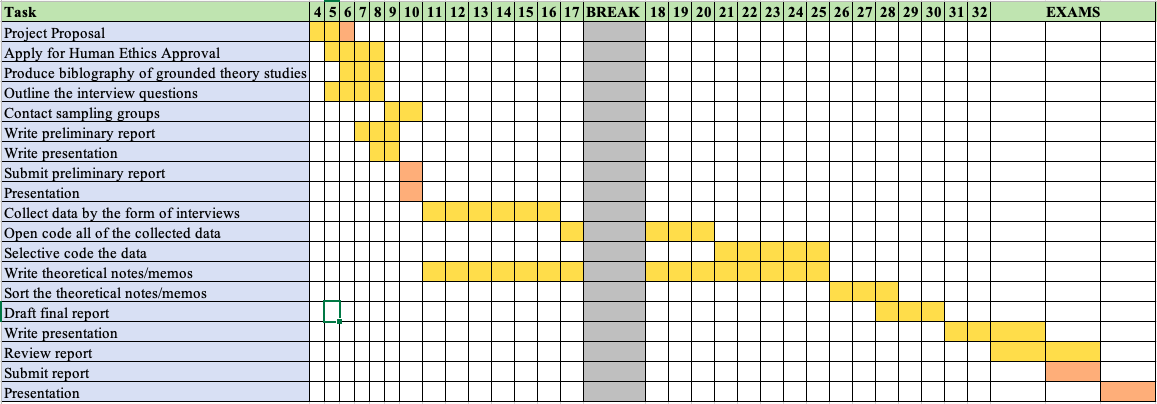
\includegraphics[width=\textwidth]{figures/fig1.png}
\newline
\newline
Above shows the Gantt chart which was outlined during the submission of the proposal. This outlined the timeline that the project would follow and what deadlines would fall within this course. 
\newline
\newline
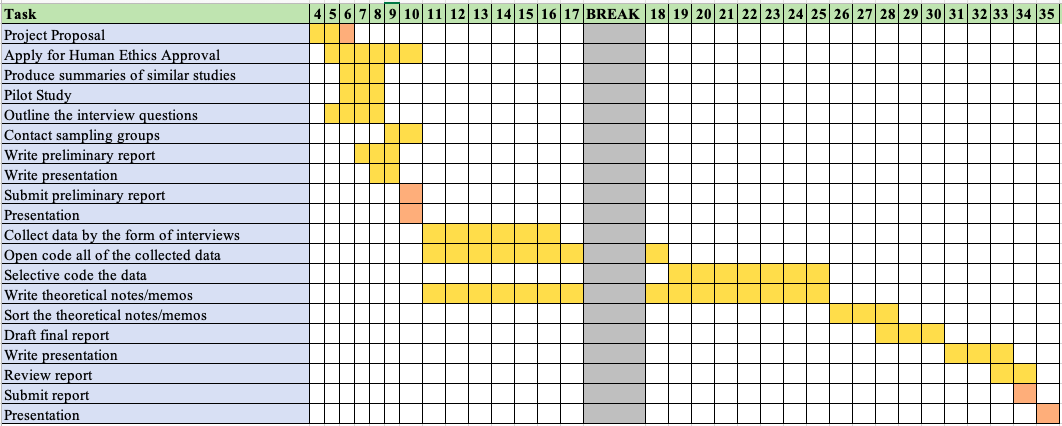
\includegraphics[width=\textwidth]{figures/fig2.png}
\newline
\newline
The above shows the now amended timeline. Not much has changed as I am following the proposed timeline quite closely. There have been additions of a pilot study which ran across weeks 6 and 7. There are still details awaiting regarding the examination period in semester two so the “EXAM” columns are amended to being week columns. The initial analysis stage of this research has also been pulled back to starting alongside the interview process as analysis will ideally occur after each interview. The entire timeline is dependent on whether the human ethics application obtains approval by the end of week 10. if this does not occur, the entire timeline will have to shift back and tasks may have to be condensed.






